% MeanFlow objective / JVP identity (meanflow_loss.py). Standardize the residual,
% sample two times r<=t, split the batch into an I-CFM diagonal part (t=r, 75%)
% and a MeanFlow off-diagonal part (r<t, 25%) whose target uses the JVP-bootstrapped
% identity u_tgt = v + (t-r) du/dr (stop-grad). The student is regressed onto the
% target with an adaptive velocity-matching loss plus a qpepre spectral penalty.
\documentclass[border=12pt]{standalone}
% Shared style for the MeanFlow thesis figures.
% Clean academic grayscale, in the spirit of the nntikz examples
% (rounded gray!10 blocks, -latex arrows). Self-contained: this does NOT
% depend on the legacy presentation/meanflow_workflow/src/mf_style.tex.
\usepackage{amsmath,amssymb,bm}
\usepackage{tikz}
\usetikzlibrary{positioning,arrows.meta,calc,fit,backgrounds,shapes.geometric,chains,decorations.pathmorphing}

\tikzset{
  % --- generic nodes ---------------------------------------------------
  base/.style    ={rounded corners=2.5pt, draw, line width=0.8pt, align=center,
                   inner sep=5pt, font=\small, text=black!88},
  block/.style   ={base, fill=gray!10},
  data/.style    ={base, fill=white},                       % data / tensors
  net/.style     ={base, fill=gray!22, line width=1.0pt},   % trained network
  frozen/.style  ={base, fill=gray!4, draw=black!60,        % frozen network
                   dash pattern=on 3pt off 2pt},
  loss/.style    ={base, fill=gray!10, line width=1.0pt,    % loss / scalar
                   double, double distance=1.2pt},
  emph/.style    ={base, fill=gray!10, line width=1.3pt},   % highlighted box
  % --- operator glyphs -------------------------------------------------
  op/.style      ={circle, draw, line width=0.8pt, fill=white,
                   minimum size=4.6mm, inner sep=0, font=\footnotesize},
  concat/.style  ={rectangle, rounded corners=1pt, draw, fill=black!72,
                   text=white, font=\scriptsize\bfseries, inner sep=2.5pt},
  % --- arrows ----------------------------------------------------------
  arrow/.style   ={-{Latex[length=2.4mm]}, line width=0.8pt, draw=black!82},
  arrowc/.style  ={arrow, rounded corners=3pt},
  thinarrow/.style={-{Latex[length=2.0mm]}, line width=0.6pt, draw=black!55},
  loopback/.style={-{Latex[length=2.4mm]}, line width=0.8pt, draw=black!55,
                   dashed, dash pattern=on 4pt off 3pt},
  % --- containers / annotation ----------------------------------------
  group/.style   ={rounded corners=5pt, draw=black!40, line width=0.7pt,
                   dashed, dash pattern=on 3pt off 2.5pt, fill=black!2,
                   inner sep=8pt},
  ttl/.style     ={font=\bfseries\large, text=black!88},
  sub/.style     ={font=\itshape\footnotesize, text=black!55},
  lab/.style     ={font=\scriptsize, text=black!70},
  tag/.style     ={font=\scriptsize\bfseries, text=black!60},
  % small sine glyph used to mark Fourier / positional embeddings
  sinewave/.style={decorate, decoration={snake, amplitude=0.6mm,
                   segment length=2.2mm}},
}

% legend swatch helper: \swatch{<style>}{<label>}
\newcommand{\swatch}[2]{%
  \tikz[baseline=-0.5ex]\node[#1, minimum width=3.6mm, minimum height=2.8mm,
    inner sep=0]{};\;#2}

\begin{document}
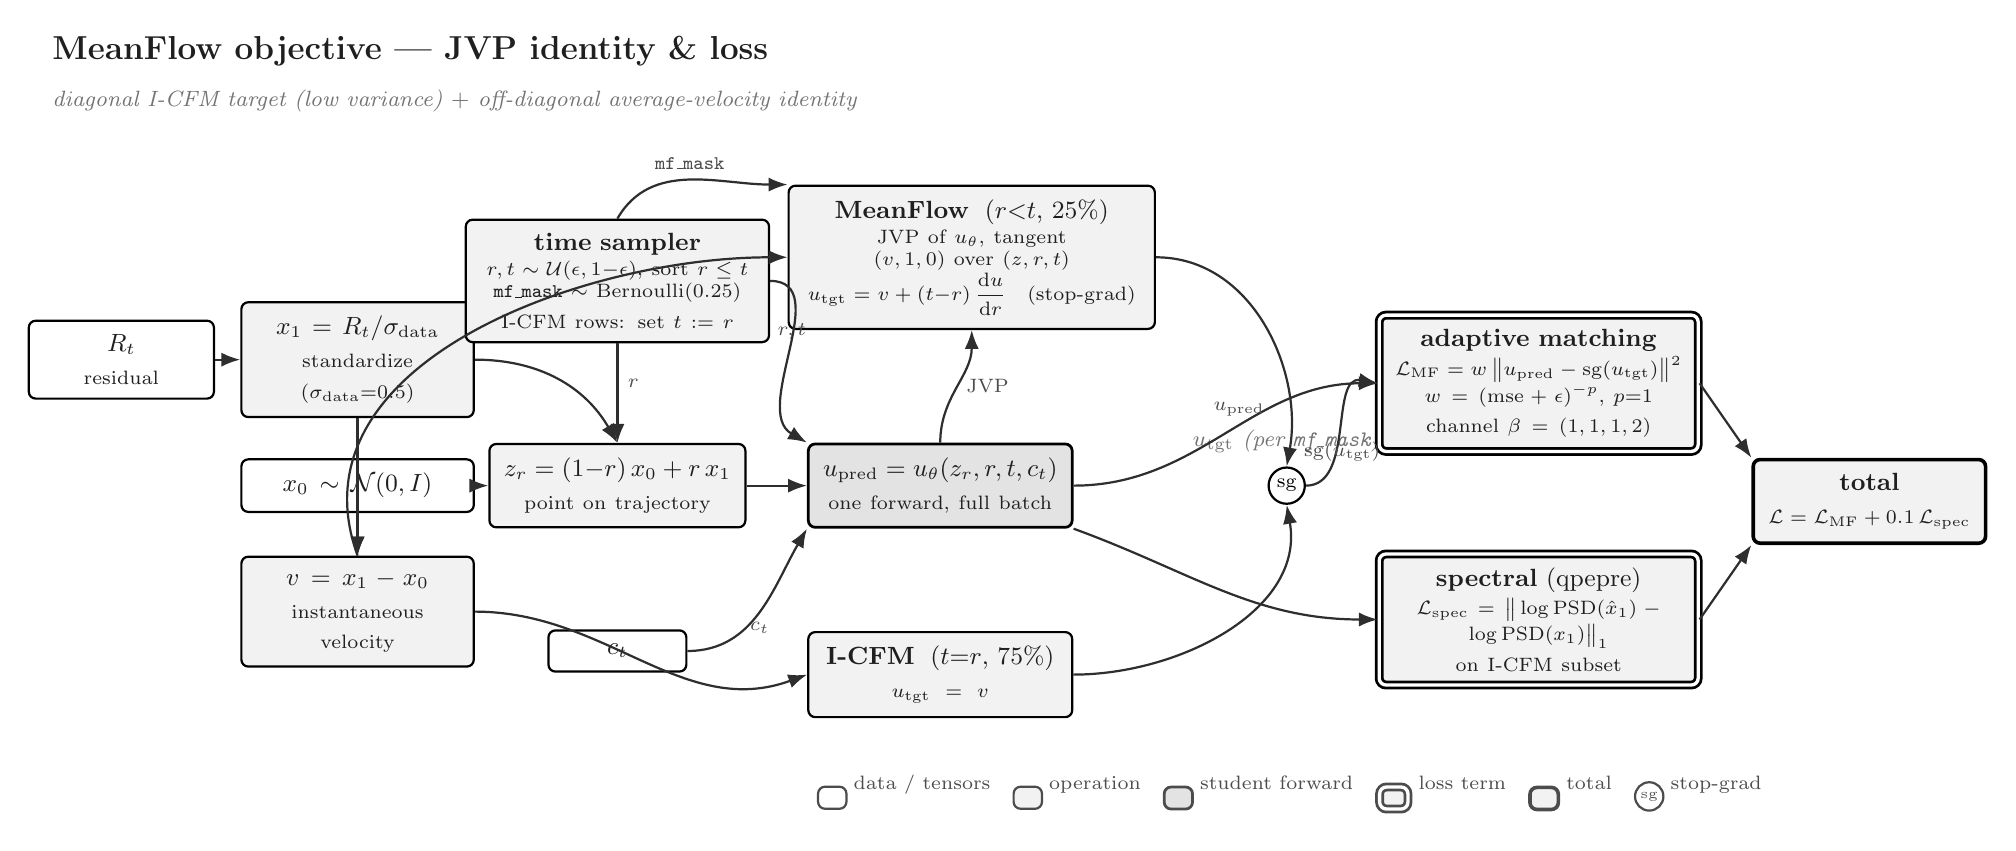
\begin{tikzpicture}[node distance=8mm]

  % ===================== flow-space setup =====================
  \node[data, text width=2.0cm] (rt) at (-2.4,1.3) {$R_t$\\[1pt]\scriptsize residual};
  \node[block, text width=2.6cm] (std) at (0.6,1.3)
    {$x_1=R_t/\sigma_{\mathrm{data}}$\\[1pt]\scriptsize standardize ($\sigma_{\mathrm{data}}{=}0.5$)};
  \node[data, text width=2.6cm] (x0) at (0.6,-0.3) {$x_0\sim\mathcal N(0,I)$};
  \node[block, text width=2.6cm] (v) at (0.6,-1.9)
    {$v=x_1-x_0$\\[1pt]\scriptsize instantaneous velocity};
  \node[block, text width=2.9cm] (zr) at (3.9,-0.3)
    {$z_r=(1{-}r)\,x_0+r\,x_1$\\[1pt]\scriptsize point on trajectory};

  % ===================== time sampler =====================
  \node[block, text width=3.5cm] (ts) at (3.9,2.3)
    {\textbf{time sampler}\\[1pt]\scriptsize $r,t\sim\mathcal U(\epsilon,1{-}\epsilon)$, sort $r\le t$\\
     $\texttt{mf\_mask}\sim\mathrm{Bernoulli}(0.25)$\\
     I-CFM rows: set $t:=r$};

  % ===================== single network forward =====================
  \node[data, text width=1.4cm] (ct) at (3.9,-2.4) {$c_t$};
  \node[net, text width=3.0cm] (up) at (8.0,-0.3)
    {\textbf{$u_{\mathrm{pred}}=u_\theta(z_r,r,t,c_t)$}\\[1pt]\scriptsize one forward, full batch};

  % ===================== target branches =====================
  \node[block, text width=4.3cm] (mf) at (8.4,2.6)
    {\textbf{MeanFlow} \;($r{<}t$, 25\%)\\[1pt]\scriptsize JVP of $u_\theta$, tangent $(v,1,0)$ over $(z,r,t)$\\
     $u_{\mathrm{tgt}}=v+(t{-}r)\,\dfrac{\mathrm{d}u}{\mathrm{d}r}$ \;\;(stop-grad)};
  \node[block, text width=3.0cm] (icfm) at (8.0,-2.7)
    {\textbf{I-CFM} \;($t{=}r$, 75\%)\\[1pt]\scriptsize $u_{\mathrm{tgt}}=v$};
  \node[op] (sw) at (12.4,-0.3) {\scriptsize sg};
  \node[sub, anchor=south] at ($(sw.north)+(0,0.5mm)$) {$u_{\mathrm{tgt}}$ (per \texttt{mf\_mask})};

  % ===================== losses =====================
  \node[loss, text width=3.7cm] (lpw) at (15.6,1.0)
    {\textbf{adaptive matching}\\[1pt]\scriptsize $\mathcal L_{\mathrm{MF}}=w\,\big\|u_{\mathrm{pred}}-\mathrm{sg}(u_{\mathrm{tgt}})\big\|^2$\\
     $w=(\mathrm{mse}+\epsilon)^{-p}$, $p{=}1$\\
     channel $\beta=(1,1,1,2)$};
  \node[loss, text width=3.7cm] (lsp) at (15.6,-2.0)
    {\textbf{spectral} (qpepre)\\[1pt]\scriptsize $\mathcal L_{\mathrm{spec}}=\big\|\log\mathrm{PSD}(\hat x_1)-\log\mathrm{PSD}(x_1)\big\|_1$\\
     on I-CFM subset};
  \node[emph, text width=2.6cm] (tot) at (19.8,-0.5)
    {\textbf{total}\\[1pt]\scriptsize $\mathcal L=\mathcal L_{\mathrm{MF}}+0.1\,\mathcal L_{\mathrm{spec}}$};

  % ===================== edges =====================
  \draw[arrow] (rt.east) -- (std.west);
  \draw[arrow] (std.south) -- (v.north);
  \draw[arrow] (x0.south) -- (v.north);
  \draw[arrow] (std.east) to[out=0,in=120] (zr.north);
  \draw[arrow] (x0.east) -- (zr.west);
  \draw[arrow] (ts.south) -- node[lab,right,pos=0.4]{$r$} (zr.north);
  \draw[arrow] (zr.east) -- (up.west);
  \draw[arrow] (ct.east) to[out=0,in=240] node[lab,below,pos=0.5]{$c_t$} (up.south west);
  \draw[arrow] (ts.east) to[out=0,in=150] node[lab,above,pos=0.5]{$r,t$} (up.north west);
  % targets
  \draw[arrow] (v.east) to[out=0,in=200] (icfm.west);
  \draw[arrow] (v.north) to[out=110,in=180] (mf.west);
  \draw[arrow] (up.north) to[out=90,in=-90] node[lab,right,pos=0.5]{JVP} (mf.south);
  \draw[arrow] (ts.north) to[out=60,in=180] node[lab,above,pos=0.5]{\texttt{mf\_mask}} (mf.north west);
  \draw[arrow] (mf.east)   to[out=0,in=80]  (sw.north);
  \draw[arrow] (icfm.east) to[out=0,in=-80] (sw.south);
  % into losses
  \draw[arrow] (up.east) to[out=0,in=180] node[lab,above,pos=0.55]{$u_{\mathrm{pred}}$} (lpw.west);
  \draw[arrow] (sw.east) to[out=0,in=170] node[lab,below,pos=0.5]{$\mathrm{sg}(u_{\mathrm{tgt}})$} (lpw.west);
  \draw[arrow] (up.south east) to[out=-20,in=180] (lsp.west);
  \draw[arrow] (lpw.east) -- (tot.north west);
  \draw[arrow] (lsp.east) -- (tot.south west);

  % ===================== title + legend =====================
  \node[ttl, anchor=south west] (title) at (-3.4,4.9)
    {MeanFlow objective --- JVP identity \& loss};
  \node[sub, anchor=north west] at ($(title.south west)+(0,-0.5mm)$)
    {diagonal I-CFM target (low variance) $+$ off-diagonal average-velocity identity};

  \node[lab, anchor=north west] at ($(icfm.south west)+(0,-0.6)$)
    {\swatch{data}{data / tensors}\quad
     \swatch{block}{operation}\quad
     \swatch{net}{student forward}\quad
     \swatch{loss}{loss term}\quad
     \swatch{emph}{total}\quad
     \tikz[baseline=-0.5ex]\node[op, minimum size=3.6mm]{\tiny sg};\;stop-grad};

\end{tikzpicture}
\end{document}
